\cleardoublepage
\chapter{PERANCANGAN}
\label{chap:perancangan}

Bab ini menjelaskan rancangan solusi yang disusun berdasarkan hasil analisis
pada Bab III: rancangan model drain baterai, arsitektur mesin simulasi,
struktur data skenario, dan rancangan dasbor visual.

Gambar~\ref{fig:arsitektur-solusi} menunjukkan arsitektur solusi yang
diusulkan. Dibandingkan dengan kondisi saat ini pada
Gambar~\ref{fig:kondisi-saat-ini} (Bab III), yang hanya terdiri atas 2 bus,
1 SPKLU, dan 1 rute tanpa mekanisme evaluasi otomatis, solusi yang
diusulkan menggantikan operasi manual tersebut dengan mesin simulasi yang
dapat menjalankan seluruh 20 koridor secara simultan, berbagai skenario
lokasi dan kapasitas SPKLU sebagai \textit{input} yang dapat diganti, serta
lapisan evaluasi (\textit{headway evaluator}) dan repetisi statistik
(Monte Carlo) yang tidak ada pada kondisi saat ini.

\begin{figure}[h]
	\centering
	\begin{tikzpicture}[
		node distance=0.9cm and 1.1cm,
		box/.style={draw, rounded corners, minimum width=3.4cm, minimum height=1cm, align=center, font=\small},
		core/.style={box, fill=blue!8},
		io/.style={box, fill=green!8},
		outbox/.style={box, fill=orange!12},
		arrow/.style={-Stealth, thick}
		]
		\node[io] (input) {Data Rute, Spesifikasi\\Bus, Skenario SPKLU};
		\node[core, below=1.0cm of input] (drain) {Battery Drain\\Model};
		\node[core, right=1.3cm of drain] (sched) {Route/Trip\\Scheduler};
		\node[core, right=1.3cm of sched] (charge) {Charging\\Decision Module};
		\node[core, below=1.0cm of sched] (spklu) {SPKLU Model\\(Antrean, $n$ gun)};
		\node[core, left=1.3cm of spklu] (evaluator) {Headway\\Evaluator};
		\node[outbox, right=1.3cm of spklu] (mc) {Monte Carlo\\Wrapper ($N$ hari)};
		\node[outbox, below=1.0cm of evaluator, xshift=1.9cm] (result) {Hasil Simulasi\\(JSON per skenario)};
		\node[outbox, below=1.0cm of result] (dash) {Dasbor Visual\\(Flask + Chart.js)};
		\draw[arrow] (input) -- (sched);
		\draw[arrow] (drain) -- (sched);
		\draw[arrow] (sched) -- (charge);
		\draw[arrow] (charge) -- (spklu);
		\draw[arrow] (sched) -- (spklu);
		\draw[arrow] (spklu) -- (evaluator);
		\draw[arrow] (evaluator) -- (result);
		\draw[arrow] (spklu) -- (mc);
		\draw[arrow] (mc) to[bend left=15] (result);
		\draw[arrow] (result) -- (dash);
		\begin{scope}[on background layer]
			\node[draw, dashed, fit=(input)(drain)(sched)(charge)(spklu)(evaluator)(mc)(result)(dash), inner sep=0.4cm] {};
		\end{scope}
	\end{tikzpicture}
	\caption{Arsitektur mesin simulasi (solusi yang diusulkan)}
	\label{fig:arsitektur-solusi}
\end{figure}

\section{Rancangan Model Drain Baterai}

Model drain baterai yang dirancang mengadopsi model konsumsi energi
non-linear dari \textcite{mamarikas2025}, yang
menyatakan konsumsi energi $EC$ (dalam Wh/km) sebagai fungsi rasional dari
kecepatan rata-rata $v$ (dalam km/jam):

\begin{equation}
	EC(v) = \frac{a v^2 + b v + c + \frac{d}{v}}{e v^2 + f v + g}
	\label{eq:ec-mamarikas}
	\eqcaption{Fungsi Konsumsi Energi $EC(v)$}
\end{equation}

dengan koefisien $a=0{,}0185$; $b=1{,}40 \times 10^{-8}$; $c=6{,}91$;
$d=1{,}54$; $e=9{,}64 \times 10^{-6}$; $f=2{,}79 \times 10^{-4}$; dan
$g=1{,}15 \times 10^{-4}$, sesuai kalibrasi asli pada paper. 
(Implementasi kode Python untuk persamaan ini selengkapnya dapat dilihat pada Lampiran A).
Model ini
dipilih secara spesifik karena sifatnya yang non-linear: konsumsi energi
terhadap kecepatan lalu
lintas, berbeda dari model heuristik awal (\textit{k1}/\textit{k2}) yang
non-linear terhadap SoC (\textit{state of charge}), yaitu persentase energi
baterai yang tersisa terhadap kapasitas penuhnya \autocite{hannan2017}.
Konsekuensinya, karakteristik drain yang melambat
atau memburuk seiring turunnya SoC baterai (fenomena fisik pada baterai
berbasis LFP) tidak lagi ditangkap secara eksplisit oleh model ini; hal ini
dicatat sebagai batasan model sebagaimana disebutkan pada Bab I.

Gambar~\ref{fig:kurva-ecv} menunjukkan bentuk kurva $EC(v)$ pada rentang
kecepatan $5$ hingga $40$ km/jam. Grafik ini dibangkitkan menggunakan pustaka \texttt{matplotlib} pada Python (melalui \textit{notebook} \texttt{lab/visualizations.ipynb}) yang langsung mengeksekusi fungsi \texttt{mamarikas\_ec()} dari modul \texttt{battery.py}. Konsumsi energi menurun tajam pada
kecepatan rendah dan melandai mendekati kecepatan optimal, mencerminkan
pemborosan energi akibat penggunaan AC yang membengkak saat bus melaju
pelan (suku $d/v$ pada Persamaan~\ref{eq:ec-mamarikas}).

\begin{figure}[h]
	\centering
	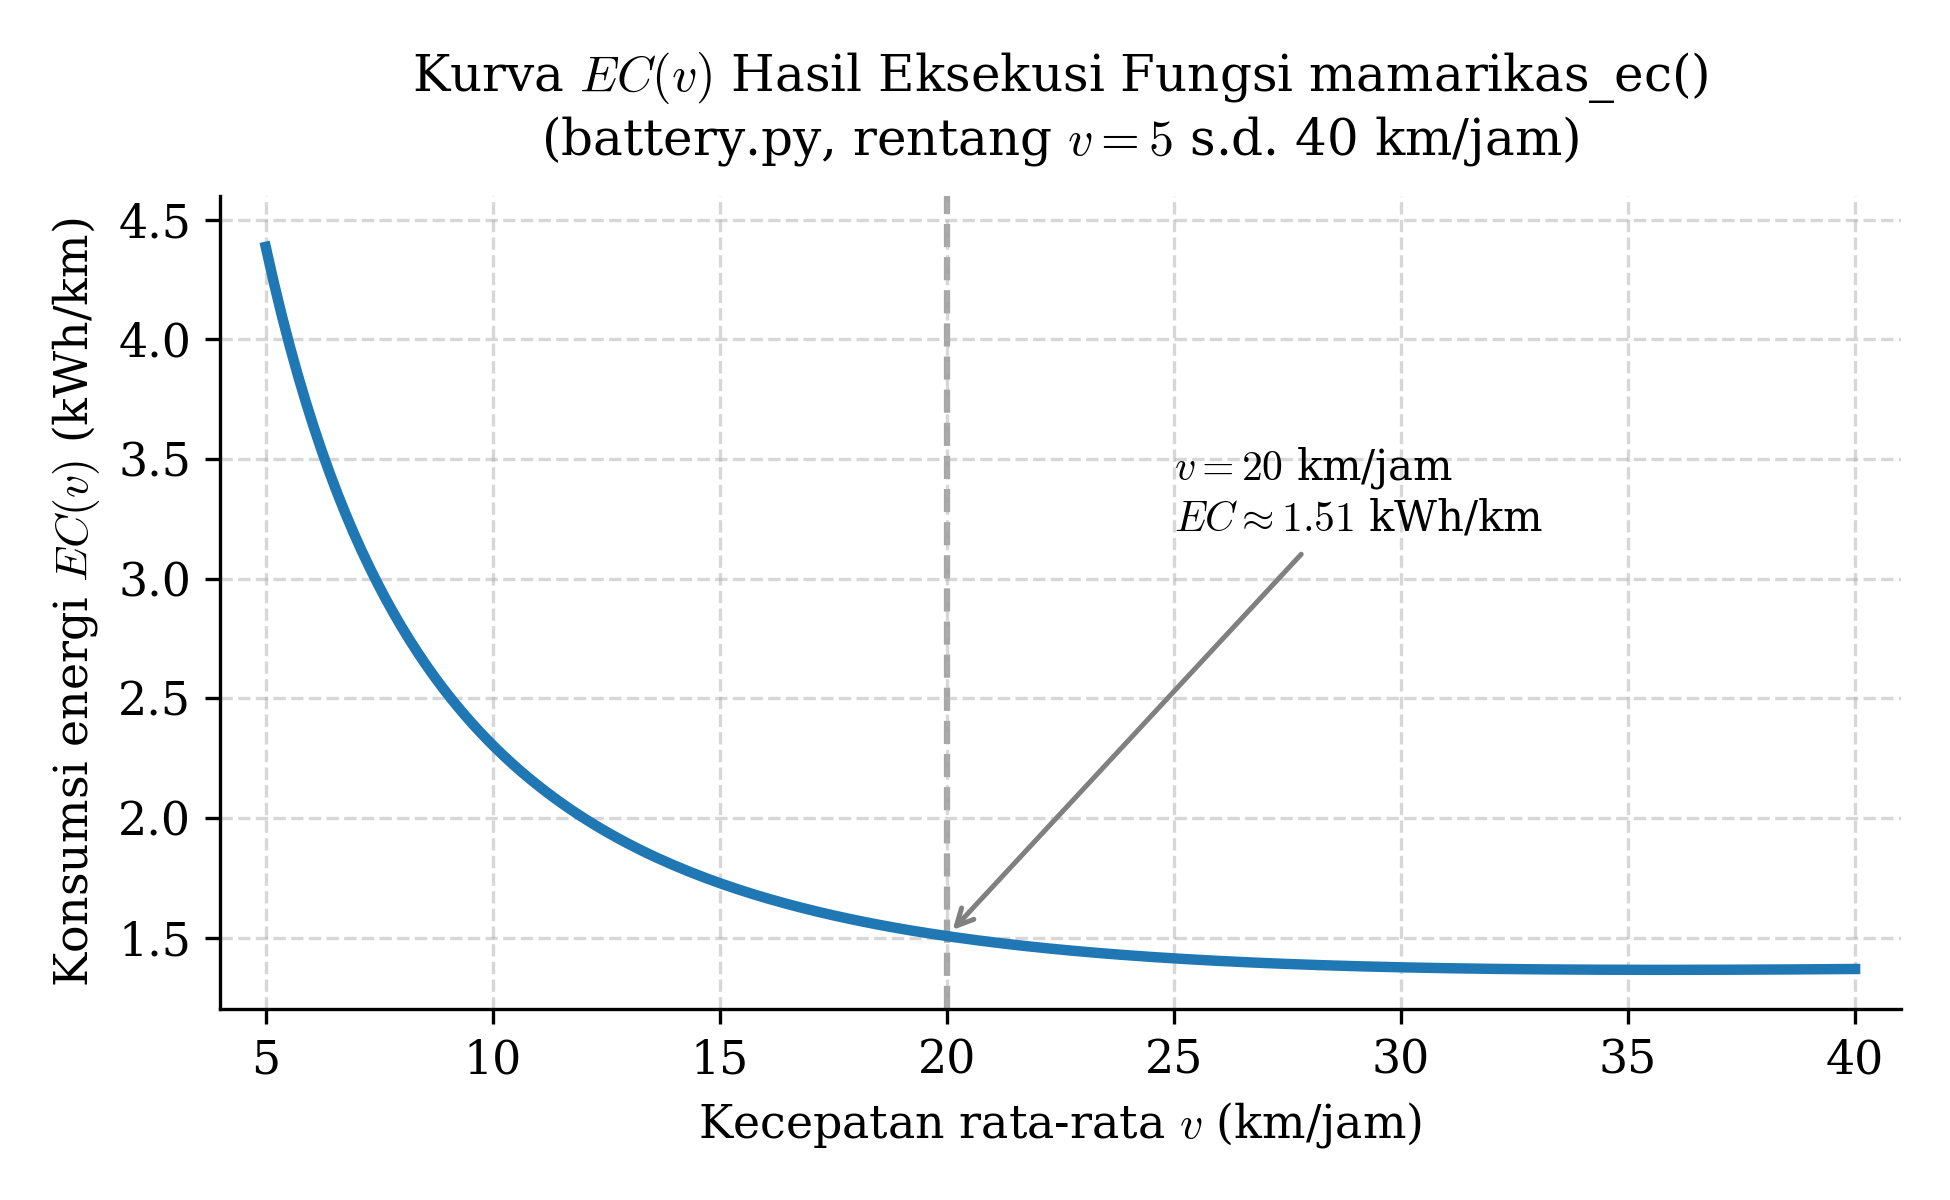
\includegraphics[width=0.75\textwidth]{images/fig_kurva_ecv.png}
	\caption{Kurva $EC(v)$ pada rentang kecepatan $5$ sampai $40$ km/jam}
	\label{fig:kurva-ecv}
\end{figure}

Paper asli melaporkan galat model ini berkisar 10\% untuk kondisi lalu
lintas urban, hingga 20\% untuk kondisi penerapan langkah manajemen lalu
lintas (\textit{traffic measures}). Paper yang sama juga menyediakan model
mesoskopik alternatif yang lebih akurat (galat 4-5\%) namun bersifat linear,
berbasis jumlah dan durasi berhenti kendaraan. Persamaan~\ref{eq:ec-mamarikas}
tetap dipilih karena sifat non-linearnya sesuai dengan arahan pembimbing;
trade-off akurasi ini adalah keputusan metodologis yang diambil secara sadar.

Nilai $EC(v)$ dari Persamaan~\ref{eq:ec-mamarikas} dikalibrasi pada paper
asli untuk bus kelas berat (16 ton, kapasitas baterai 250-350 kWh), sedangkan
bus TransJogja adalah bus kelas menengah dengan kapasitas baterai sekitar
138,87 kWh (titik tengah rentang spesifikasi 127,74-150 kWh). Akibatnya,
hasil perhitungan Persamaan~\ref{eq:ec-mamarikas} menghasilkan konsumsi
energi yang lebih tinggi dari kondisi riil TransJogja, sehingga kebutuhan
pengisian daya harian pada baseline Rute L-1 bergeser dari 2 sesi/hari
(kondisi riil) menjadi 3 sesi/hari pada hasil simulasi. Faktor skala
buatan (\textit{fudge factor}) untuk menyesuaikan hasil ke kondisi riil
sengaja tidak diterapkan, karena penyesuaian semacam itu akan merusak
validitas kutipan model literatur tanpa dukungan data primer yang memadai
untuk menentukan besarannya. Deviasi ini dicatat sebagai batasan akurasi
model, konsisten dengan Bab I.

SoC tiap bus dihitung mundur sepanjang rit
berdasarkan energi yang terpakai per segmen jarak antar-halte:

\begin{equation}
	SoC_i = SoC_{i-1} - \frac{EC(v_i) \times d_i}{E_{bat}} \times 100\%
	\label{eq:soc-update}
	\eqcaption{Pembaruan \textit{State of Charge} (SoC) Tiap Segmen}
\end{equation}

dengan $d_i$ adalah jarak segmen ke-$i$ (km), $v_i$ adalah kecepatan
rata-rata pada segmen tersebut, dan $E_{bat}$ adalah kapasitas baterai
(kWh). Bus mulai mencari SPKLU untuk mengisi daya saat $SoC \leq 30\%$, dan
sistem mencatat pelanggaran apabila $SoC$ menyentuh ambang keras $20\%$
(yaitu kondisi saat AC bus mati, dihindari pada operasi normal).

\subsection{Sifat Non-Linear dan Pengaruh \textit{Jensen's Inequality}}

Bentuk Fungsi Rasional Polinomial pada Persamaan~\ref{eq:ec-mamarikas}
mengakibatkan tingkat pengurasan baterai (\textit{drain}) dalam simulasi
bersifat non-linear terhadap kecepatan. Faktor kuadratik ($v^2$) pada
pembilang merepresentasikan hambatan aerodinamis yang meningkat secara
eksponensial pada kecepatan tinggi, sedangkan faktor pembagi ($d/v$)
merepresentasikan pemborosan energi diam (seperti AC) yang dominan saat bus
terjebak kemacetan. Karena fungsi ini berbentuk cembung (membentuk kurva U)
dengan titik optimal di sekitar 35 km/jam, berlakulah hukum \textit{Jensen's Inequality}
secara matematis: nilai rata-rata dari fungsi terhadap kecepatan acak selalu
lebih besar dari nilai fungsi terhadap kecepatan rata-rata ($E[EC(v)] > EC(E[v])$).

Artinya, fluktuasi kecepatan antara berhenti total dan melaju akibat
kemacetan menghasilkan konsumsi energi yang selalu lebih tinggi dibanding
laju konstan, meskipun kecepatan rata-ratanya sama. Validasi awal pada
mesin simulasi terhadap 360.000 segmen sintetis membuktikan hal ini: bus yang
melaju konstan 20 km/jam mengonsumsi rata-rata 1,49 kWh/km, sedangkan bus
yang berfluktuasi dengan kecepatan rata-rata akhir 20 km/jam mengonsumsi
1,51 kWh/km (terdapat penalti pemborosan non-linear sebesar +1,49\%).
Karakteristik mikroskopik inilah yang membedakan simulasi harian fisik ini
dari model kalkulasi agregat.

\section{Rancangan Randomisasi Waktu Tempuh}

Untuk menangkap variasi kondisi lalu lintas harian, kecepatan tempuh
dirancang sebagai variabel acak berdistribusi log-normal terpotong, dengan
dua tingkat variasi:
\begin{enumerate}
	\item \textbf{Modifier harian} (\textit{Coefficient of Variation},
	$CV=15\%$): satu nilai acak yang berlaku
	untuk seluruh rute pada hari simulasi yang sama, merepresentasikan kondisi
	kemacetan kota yang bersifat sistemik (memengaruhi banyak rute sekaligus,
	bukan terisolasi pada satu rute).
	\item \textbf{Residual per-segmen} ($CV=5\%$): variasi tambahan pada
	tingkat segmen individual di atas \textit{modifier} harian.
\end{enumerate}
Kecepatan rata-rata dasar ditetapkan 20 km/jam, yang ditransformasikan menjadi waktu tempuh dasar $t_{\text{base}}$. Waktu tempuh aktual tiap segmen $t_{\text{aktual}}$ dimodelkan mengikuti distribusi probabilitas \textit{log-normal} terpotong (\textit{truncated log-normal}) sesuai Persamaan~\ref{eq:lognormal-time}:

\begin{equation} \label{eq:lognormal-time}
\begin{aligned}
    t_{\text{expected}} &= t_{\text{base}} \times M_{\text{daily}} \\
    \sigma &= \sqrt{\ln(1 + CV_{\text{seg}}^2)} \\
    \mu &= \ln(t_{\text{expected}}) - \frac{\sigma^2}{2} \\
    t_{\text{aktual}} &\sim \text{Lognormal}(\mu, \sigma) \\
    \text{dengan batasan: } & \left(\frac{d}{40 \text{ km/jam}}\right) \leq t_{\text{aktual}} \leq \left(\frac{d}{5 \text{ km/jam}}\right)
\end{aligned}
\eqcaption{Model Waktu Tempuh Segmen Terandomisasi dengan Distribusi \textit{Log-normal}}
\end{equation}

Batas bawah (berkorespondensi dengan 40 km/jam) mencegah suku $d/v$ pada Persamaan~\ref{eq:ec-mamarikas} mengecil secara ekstrem, dan batas atas (berkorespondensi dengan 5 km/jam) mencegah waktu tempuh melonjak tidak wajar dan memastikan konsistensi dengan rentang kalibrasi asli model kecepatan \autocite{mamarikas2025}.

\section{Rancangan Arsitektur Mesin Simulasi}

Mesin simulasi dirancang berbasis peristiwa diskrit (\textit{Discrete Event
	Simulation}), menggunakan antrean prioritas untuk memproses peristiwa
berdasarkan urutan waktu kejadian. Arsitektur ini dipisahkan dari lapisan
visualisasi melalui satu berkas hasil (\texttt{simulation\_result.json})
per skenario, sehingga mesin simulasi dapat dijalankan secara
\textit{headless} (tanpa antarmuka) untuk menjalankan banyak skenario
sekaligus, dan dasbor cukup membaca hasil yang sudah tersimpan.

Mesin simulasi terdiri atas lima komponen utama:
\begin{enumerate}
	\item \textbf{Battery Drain Model}: menghitung SoC sepanjang rit
	berdasarkan Persamaan~\ref{eq:ec-mamarikas} dan \ref{eq:soc-update}.
	\item \textbf{Route/Trip Scheduler}: menjadwalkan rit berulang tiap bus
	sepanjang jam operasional (05.30-20.30), sesuai jumlah bus dan target
	headway per koridor.
	\item \textbf{Charging Decision Module}: menentukan waktu dan lokasi
	pengisian daya bus, sesuai mekanisme skenario aktif (\textit{opportunity},
	\textit{depot}, \textit{mix}, atau dinamis).
	\item \textbf{SPKLU Model}: merepresentasikan tiap titik SPKLU sebagai
	\textit{resource} dengan kapasitas terbatas (jumlah \textit{gun} --
	konektor/colokan pengisian daya individual dalam satu SPKLU), antrean FIFO
	(\textit{first-in-first-out}), dan waktu layanan berupa durasi
	pengisian daya.
	\item \textbf{Headway Evaluator}: menghitung kinerja layanan berdasarkan realisasi keberangkatan. \textit{Headway} rata-rata $\bar{h}_r$ dan deviasinya terhadap target Dishub $\Delta h_r$ dirumuskan pada Persamaan~\ref{eq:headway-dev}:
\begin{equation} \label{eq:headway-dev}
\begin{aligned}
    \bar{h}_r &= \frac{1}{N_r - 1} \sum_{i=2}^{N_r} (t_{i,r} - t_{i-1,r}) \\
    \Delta h_r &= \bar{h}_r - h_{\text{target}, r}
\end{aligned}
\eqcaption{Deviasi \textit{Headway} Rata-Rata terhadap Target Operasional}
\end{equation}
dengan $t_{i,r}$ adalah waktu keberangkatan rit ke-$i$ pada rute $r$, dan $N_r$ adalah total rit terselesaikan. Selain itu, evaluator ini menentukan status kelumpuhan operasional (\textit{degraded route}) sesuai Persamaan~\ref{eq:degraded-route}:
\begin{equation} \label{eq:degraded-route}
    \text{Status}(r) = 
    \begin{cases} 
        \text{Lumpuh}, & \exists b \in B_r : SoC_b \leq 20\% \lor \\
                       & \left( w_{q,b} \geq 30\text{ mnt} \land t_{\text{cas}} \geq t_{\text{akhir\_shift}} \right) \\
        \text{Normal}, & \text{lainnya}
    \end{cases}
\eqcaption{Kriteria Kelumpuhan Operasional (\textit{Degraded Route})}
\end{equation}
Rute $r$ dianggap lumpuh terdegradasi jika setidaknya satu armada bus $b$ di rute tersebut mogok di jalan akibat kehabisan daya (menembus \textit{hard limit} 20\%) atau membatalkan pengisian daya karena durasi antrean SPKLU $w_{q,b} \geq 30$ menit yang menyebabkan waktu mulai pengisian daya ($t_{\text{cas}}$) terdorong hingga melewati batas akhir jam operasional ($t_{\text{akhir\_shift}}$).
\end{enumerate}

Gambar~\ref{fig:state-bus} menunjukkan diagram status (\textit{state
	diagram}) siklus operasi tiap bus dalam mesin simulasi, mulai dari bus
diam di \textit{pool} hingga kembali beroperasi setelah mengisi daya atau
berakhir shift.

\begin{figure}[h]
	\centering
	\begin{tikzpicture}[
		node distance=1.1cm and 1.5cm,
		state/.style={draw, rounded corners, minimum width=3.0cm, minimum height=0.9cm, align=center, font=\small},
		decision/.style={draw, diamond, aspect=2.2, align=center, font=\scriptsize, inner sep=2pt, fill=yellow!12},
		startstop/.style={state, fill=gray!12},
		arrow/.style={-Stealth, thick},
		lbl/.style={font=\scriptsize\itshape}
		]
		\node[startstop] (idle) {IDLE\_AT\_POOL};
		\node[state, right=of idle] (route) {EN\_ROUTE};
		\node[decision, below=1.0cm of route] (cek) {SoC\\$\leq 30\%$?};
		\node[state, right=1.3cm of cek] (travel) {TRAVEL\_TO\_SPKLU};
		\node[state, below=of travel] (charge) {CHARGING};
		\node[decision, below=1.0cm of route, xshift=-4.6cm] (akhir) {Akhir\\shift?};
		\node[state, below=of akhir] (pool) {RETURN\_TO\_POOL};
		\node[state, below=of pool] (depot) {DEPOT\_CHARGING};
		\draw[arrow] (idle) -- (route);
		\draw[arrow] (route.south) -- (cek.north);
		\draw[arrow] (cek) -- node[above, lbl]{ya} (travel);
		\draw[arrow] (travel) -- (charge);
		\draw[arrow] (charge.west) to[bend right=20] node[below, lbl, pos=0.4]{lanjut rit} (route.south east);
		\draw[arrow] (cek.west) -- node[above, lbl]{tidak} (akhir.east);
		\draw[arrow] (akhir) -- node[left, lbl]{ya} (pool);
		\draw[arrow] (pool) -- (depot);
		\draw[arrow] (akhir.north) to[bend right=25] node[above, lbl, pos=0.6]{tidak, lanjut rit} (route.south west);
	\end{tikzpicture}
	\caption{Diagram status siklus operasi bus dalam mesin simulasi}
	\label{fig:state-bus}
\end{figure}

\subsection{Mekanisme Pengisian Daya}

Tiga mekanisme dasar dirancang untuk dapat dibandingkan sebagai skenario:
\begin{enumerate}
	\item \textbf{Full opportunity charging}: bus mengisi daya di SPKLU
	sepanjang rute saat $SoC \leq 30\%$; bus tambahan (bila dikonfigurasi)
	menutup slot headway yang kosong saat 1 bus keluar untuk mengisi daya.
	\item \textbf{Full depot charging}: bus hanya mengisi daya penuh di
	pool/depot (Banguntapan atau Gamping, sesuai pemetaan pool-koridor),
	tanpa pengisian daya di jalan.
	\item \textbf{Mix}: kombinasi \textit{opportunity} dan \textit{depot
		charging}, dengan opsi penambahan bus per koridor.
\end{enumerate}
Karena simulasi bersifat harian dan berdiri sendiri per hari (lihat Bab I,
Batasan Masalah), mekanisme \textit{mix} secara struktural menghasilkan
metrik headway siang hari yang identik dengan \textit{full opportunity
	charging}, karena pengisian daya di depot terjadi di luar jendela waktu
operasional yang diukur.

Selain ketiga mekanisme dasar, dirancang pula modul pengisian daya dinamis
yang menyesuaikan target SoC pengisian berdasarkan kondisi operasional,
dengan dua varian:
\begin{enumerate}
	\item \textbf{V1 (\textit{time-aware})}: memotong target SoC pengisian ke
	80\% apabila sesi pengisian bertumpang tindih dengan jam sibuk (durasi
	tumpang tindih $\geq 15$ menit).
	\item \textbf{V2 (\textit{queue-aware})}: memotong target SoC pengisian
	berdasarkan proyeksi antrean nyata di SPKLU tujuan (dihitung melalui
	simulasi bayangan/\textit{shadow simulation} kondisi \textit{in-transit}),
	bukan berdasarkan waktu.
\end{enumerate}

\begin{algorithm}[h]
\caption{Algoritma Pengisian Daya Dinamis V1 (\textit{Time-aware})}
\label{alg:dinamis-v1}
\begin{algorithmic}[1]
\Require Waktu kedatangan bus $T_{datang}$, Durasi normal $D_{normal}$, Jam Sibuk $JS$
\Ensure Target SoC (100\% atau 80\%)
\State $T_{selesai} \gets T_{datang} + D_{normal}$
\State $D_{overlap} \gets$ HitungTumpangTindihWaktu($[T_{datang}, T_{selesai}]$, $JS$)
\If{$D_{overlap} \geq 15$ menit}
    \State \Return 80\%
\Else
    \State \Return 100\%
\EndIf
\end{algorithmic}
\end{algorithm}

\begin{algorithm}[h]
\caption{Algoritma Pengisian Daya Dinamis V2 (\textit{Queue-aware})}
\label{alg:dinamis-v2}
\begin{algorithmic}[1]
\Require Status antrean SPKLU saat ini $Q_{spklu}$, Bus lain yang menuju SPKLU $B_{transit}$
\Ensure Target SoC (100\% atau 80\%)
\State $Q_{proyeksi} \gets Q_{spklu}$
\For{setiap bus $b \in B_{transit}$}
    \If{WaktuKedatangan($b$) $\approx$ WaktuKedatangan(BusSekarang)}
        \State $Q_{proyeksi} \gets Q_{proyeksi} + 1$
    \EndIf
\EndFor
\If{$Q_{proyeksi} \geq$ Kapasitas SPKLU}
    \State \Return 80\%
\Else
    \State \Return 100\%
\EndIf
\end{algorithmic}
\end{algorithm}

Hasil pengujian kedua varian ini terhadap headway dan tingkat kegagalan
rute dijelaskan pada Bab VI.

\subsection{Simulasi Stokastik Monte Carlo}

Untuk menangkap variasi hasil akibat randomisasi waktu tempuh, dirancang
lapisan pembungkus (\textit{wrapper}) Monte Carlo di luar mesin simulasi
inti: mesin simulasi dijalankan berulang sejumlah $N$ hari independen
dengan \textit{random seed} yang berbeda dan terdokumentasi pada tiap
repetisi, kemudian hasilnya diringkas secara statistik (rata-rata dan
deviasi standar) per skenario. Nilai rata-rata headway konvergen pada
$N=50$ (selisih di bawah 2\% terhadap nilai pada $N=100$). Namun,
deviasi standar belum stabil pada $N=50$: distribusi headway berekor
panjang (\textit{long-tailed}) akibat efek berantai penumpukan bus
(\textit{bus bunching}) pada hari-hari dengan kondisi lalu lintas buruk,
sehingga kejadian-kejadian ekstrem yang langka baru mulai tertangkap
secara memadai di atas $N=50$ repetisi. Atas dasar ini, $N=100$
ditetapkan sebagai jumlah repetisi baku untuk seluruh skenario evaluasi,
agar deviasi standar headway juga terukur secara valid. Hasil pengujian
konvergensi secara lengkap dilaporkan pada Bab~VI.

\section{Rancangan Struktur Data Skenario}

Tiap skenario dirancang sebagai satu berkas konfigurasi
(\url{data/scenarios/<nama>.json}) yang mendefinisikan mekanisme
pengisian daya, lokasi dan kapasitas SPKLU yang digunakan, serta parameter
tambahan seperti penggunaan bus tambahan per koridor dan pengisian daya
dinamis. Gambar~\ref{fig:struktur-data} menunjukkan relasi konseptual
antar-bagian struktur data ini, sebelum ditunjukkan struktur JSON
lengkapnya pada Listing~\ref{lst:scenario-schema}.

\begin{figure}[h]
	\centering
	\begin{tikzpicture}[
		main/.style={draw, rounded corners, minimum width=4.4cm, minimum height=1cm, align=center, font=\small\bfseries, fill=gray!10},
		sub/.style={draw, rounded corners, align=left, font=\scriptsize, fill=blue!8, text width=5.2cm, inner sep=8pt},
		key/.style={draw, rounded corners, minimum width=3.2cm, minimum height=0.8cm, align=center, font=\scriptsize\ttfamily, fill=orange!12},
		arrow/.style={-Stealth, thick},
		lbl/.style={font=\scriptsize\itshape}
		]
		\node[main] (scenario) at (0, 6) {Konfigurasi Skenario\\(1 berkas JSON)};
		\node[sub] (assign) at (-3.6, 3.3) {
			\texttt{spklu\_assignment\_map}\\[3pt]
			\{ Rute $\rightarrow$ Kode SPKLU \}\\[3pt]
			\textit{contoh:} "1A" $\rightarrow$ "SPKLU-ADI"
		};
		\node[sub] (details) at (3.6, 3.3) {
			\texttt{spklu\_details}\\[3pt]
			\{ Kode SPKLU $\rightarrow$ kapasitas \}\\[3pt]
			\textit{contoh:} "SPKLU-ADI" $\rightarrow$\\
			\{n\_gun, travel\_min, charge\_min\}
		};
		\node[key] (joinkey) at (0, 0.7) {Kode SPKLU\\(kunci penghubung)};
		\draw[arrow] (scenario) -- (assign);
		\draw[arrow] (scenario) -- (details);
		\draw[arrow, dashed] (assign.south) -- node[left, lbl, pos=0.55]{sumbu lokasi} (joinkey.north west);
		\draw[arrow, dashed] (details.south) -- node[right, lbl, pos=0.55]{sumbu kapasitas} (joinkey.north east);
		\node[align=center, font=\scriptsize, text width=10.5cm] (note) at (0, -0.9)
		{Kedua sumbu dapat diubah independen: mengganti lokasi
			(\texttt{assignment\_map}) tidak mengubah nilai kapasitas
			(\texttt{details}), begitu pula sebaliknya.};
	\end{tikzpicture}
	\caption{Relasi konseptual struktur data konfigurasi skenario}
	\label{fig:struktur-data}
\end{figure}

\newpage
Struktur JSON ringkasnya adalah sebagai berikut:

\begin{lstlisting}[caption=Struktur konfigurasi skenario (disederhanakan), label=lst:scenario-schema]
	{
		"scenario_id": "s17b_probabilistic_4loc_prop",
		"charging_mechanism": "full_opportunity",
		"extra_bus_per_route": 0,
		"dynamic_charging": false,
		"spklu_assignment_map": {
			"SPKLU-ADI": ["1A", "14"],
			"SPKLU-NGB": ["1B", "3B", "6", "9", "10", "11", "13", "15"]
		},
		"spklu_details": {
			"SPKLU-ADI": { "n_gun": 2, "travel_min": 60, "charge_min": 60 },
			"SPKLU-NGB": { "n_gun": 8, "travel_min": 30, "charge_min": 60 }
		}
	}
\end{lstlisting}

Pemisahan \texttt{spklu\_assignment\_map} (koridor mana dilayani SPKLU mana)
dari \texttt{spklu\_details} (kapasitas gun dan waktu tempuh/pengisian tiap
SPKLU) dirancang agar kedua aspek ini, lokasi dan kapasitas, dapat diuji
sebagai dua sumbu skenario yang independen satu sama lain tanpa mengubah
struktur data secara keseluruhan.

\section{Rancangan Dasbor Visual}

Dasbor visual dirancang sebagai aplikasi web ringan yang membaca hasil
simulasi yang sudah tersimpan, tanpa menjalankan ulang logika simulasi di
sisi klien. Rancangan ini terdiri atas:
\begin{enumerate}
	\item \textbf{Peta skematik rute}: direpresentasikan sebagai SVG generatif
	yang dibangun dari data urutan halte tiap koridor, mengacu pada peta rute
	resmi TransJogja sebagai referensi visual.
	\item \textbf{Panel pemutaran (\textit{playback})}: menampilkan animasi
	pergerakan bus dan perubahan SoC sepanjang waktu simulasi untuk skenario
	yang dipilih.
	\item \textbf{Panel pemilihan skenario}: memungkinkan pembaca berpindah
	antar-skenario untuk dibandingkan.
	\item \textbf{Panel metrik hasil}: menampilkan ringkasan headway aktual
	terhadap target, jumlah rute yang mengalami kegagalan, dan metrik antrean
	SPKLU per skenario.
\end{enumerate}
Rancangan ini mengikuti prinsip keterpisahan (Bab III, Kebutuhan
Nonfungsional): \textit{backend} menyajikan data hasil simulasi sebagai
JSON, sedangkan \textit{frontend} menerjemahkannya menjadi visual tanpa
proses \textit{build} tambahan, sesuai hasil analisis pemilihan teknologi
dasbor pada Bab III.